\documentclass[tikz,border=6pt]{standalone}
\usepackage{tikz}
\usetikzlibrary{arrows.meta,angles,quotes}

\begin{document}
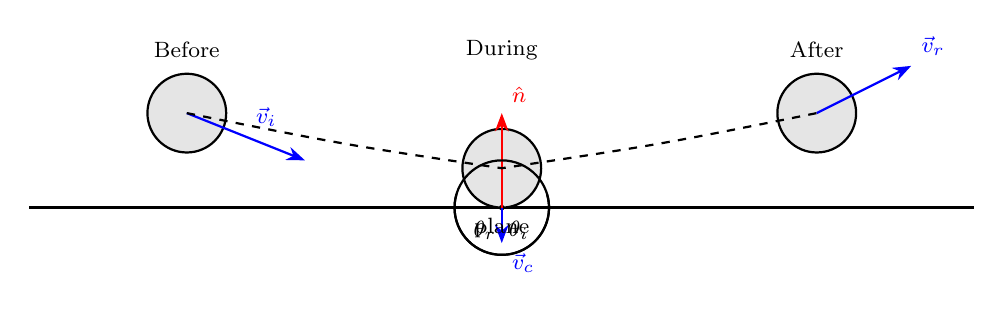
\begin{tikzpicture}[
    thick,
    every node/.style={font=\footnotesize},
    >=Stealth
]

% Plane
\draw[very thick] (0,0) -- (12,0);

% Centers (three states)
\coordinate (B) at (2,1.2);   % before
\coordinate (C) at (6,0.5);   % during (contact)
\coordinate (A) at (10,1.2);  % after

\def\r{0.5}

% Spheres
\fill[gray!20] (B) circle (\r); \draw (B) circle (\r);
\fill[gray!20] (C) circle (\r); \draw (C) circle (\r);
\fill[gray!20] (A) circle (\r); \draw (A) circle (\r);

% Contact point (foot on plane) and normal reference point
\coordinate (P) at (6,0);      % contact point on plane
\coordinate (N) at (6,1.2);    % point along the normal above contact

\fill (P) circle (1pt);

% Velocity vectors (incoming, at contact, reflected)
\draw[->, blue] (B) -- ++(1.5,-0.6) node[midway, above right] {$\vec v_i$};
\draw[->, blue] (C) -- ++(0,-0.95) node[below right] {$\vec v_c$};
\draw[->, blue] (A) -- ++(1.2,0.6) node[above right] {$\vec v_r$};

% Normal at contact
\draw[red,->] (P) -- (N) node[above right] {$\hat n$};

% Angle markers using the `angles` pic (robust)
\pic["$\theta_i$", draw=black, angle radius=6mm] {angle = B--P--N};
\pic["$\theta_r$", draw=black, angle radius=6mm] {angle = N--P--A};

% Dashed trajectory through the contact (visual guide)
\draw[dashed] (B) .. controls (4,0.8) .. (C) .. controls (8,0.8) .. (A);

% Phase labels
\node at (2,2)  {Before};
\node at (6,2)  {During};
\node at (10,2) {After};

\node[below] at (6,0) {plane};

\end{tikzpicture}
\end{document}